\documentclass{udthesis}

\usepackage[english]{babel}
%\usepackage{float}
%\usepackage[hidelinks]{hyperref}
\usepackage{graphicx}
\usepackage{bookmark}

\makeatletter
\providecommand{\toclevel@prefacesection}{0}
\makeatother 

\usepackage[usenames,dvipsnames]{xcolor}
\usepackage{tcolorbox}
\usepackage{tabularx}
\usepackage{array}
\usepackage{colortbl}
\tcbuselibrary{skins}

\pdfoptionpdfminorversion=7

\newcolumntype{Y}{>{\raggedleft\arraybackslash}X}
\definecolor{myblue}{RGB}{72,107,123}
\definecolor{myblue2}{RGB}{184,206,216}

\tcbset{borderline={0.5mm}{0.0mm}{myblue},sharp corners,width=10cm,enhanced,boxrule=0.5pt,fonttitle=\normalsize,
colback=gray!01!white,colframe=myblue,colbacktitle=myblue2,
coltitle=black,center title,shrink tight}

%\usepackage{draftwatermark}
%\SetWatermarkScale{8}
%\SetWatermarkLightness{0.96}

\begin{document}
    %FIXME: FIX NUMBERING of pages to romane numerals, Get required pages (see Josh's thesis), add Acknowledgment.
    \title[An Experimental Exploration of Self-aware Systems for Exascale Architectures]{An Experimental Exploration of Self-aware Systems for Exascale Architectures}
                   % This file (thesis-tap.tex) contains the Title
                   % and Approval Page information for a master's thesis.

    \author{Aaron Myles Landwehr}
    \type{thesis}
    \degree{Master of Science in Electrical and Computer Engineering}
    \majorfieldtrue\majorfield{Electrical \& Computer Engineering}
    \degreedate{Summer 2016}
    \keywords{self-awareness, self-adaptation, exascale architectures}
    \subject{Subject}

    \maketitlepage

    \begin{approvalpage}
    \prof{Guang R. Gao, Ph.D.}
    \chair{Kenneth E. Barner, Ph.D.}{Chair of the Department of Electrical \& Computer Engineering}
    \dean{Babatunde A. Ogunnaike, Ph.D.}{Dean of the College of Engineering}
    \end{approvalpage}

    \begin{front} % Starts front material (Roman style page numbers)
        \prefacesection{Acknowledgments}
            \input{Text/acknowledgments}

        \tablespagefalse 
        \maketocloflot
        \prefacesectiontoc{Abstract}
            %As we move toward an exascale future with ever expanding capacities in terms of both cores and resources, we have reached a point in high performance computing where current execution paradigms will no-longer suffice. With the multiplicity of transistors and components comes ever increasing power requirements which necessarily result in the need for a fundamental and radical shift in both terms of programmability and adaptation. We believe that system runtimes will need to become hierarchically introspective and self-aware to be able adapt to the steep performance and energy requirements of these future systems. To this end, this document explores the major hardware requirements we believe are central to enabling introspection, the types of interfaces and information that will be needed for introspective system runtimes, and discusses a research path toward a self-aware system for exascale architectures.      

High-performance systems are evolving to a point where performance is no longer the sole relevant criterion anymore. Current execution and resource management paradigms are no longer sufficient to ensure correctness and performance. Power requirements are presently driving the co-design of HPC systems, which in turn sets the course for a radical change in how to express the need for scarcer and scarcer resources, as well as, how to manage them. As a result, systems will need to become more introspective and self-aware with respect to performance, energy, and resiliency. To this end, this thesis explores the major hardware requirements that are central to enabling introspection, the types of interfaces and information that will be needed for introspective system software, provides an abstract representation of exascale architectures based on current trends, and implements an exascale simulation framework with built in temperature and power management capabilities. Through this framework, we demonstrate that localized adaptive policies are not sufficient for exascale systems and that instead coordinated hierarchical adaptive policies are need in order to effectively adapt and mitigate oscillation within systems consisting of thousands of independent cores.

    \end{front}

    \pagenumbering{arabic}

    \chapter{Introduction}
        \label{chap:introduction}

%Cite me: Architectural Aspects of Self-Aware and Self-Expressive Computing Systems: From Psychology to Engineering~\cite{LewisEtAl2015}. %It can be a good paper to cite in your intro, to give a broader sense of what people think when we mention self-awareness, then you can narrow the focus in your contributions and in the background.

%Cite me in discussion of self-awareness: Revisiting Goal-Oriented Models for Self-Aware Systems-of-Systems\cite{CavalcanteEtAl2015}.

%Cite me in discussion of self-awareness: Self-Aware and Self-Expressive Systems~\cite{TorresenEtAl2015}.

%Cite me in discussion of self-awareness: Self-aware architecture to support partial control of emergent behavior~\cite{MotusEtAl2012}.

As we move toward an exascale future with ever expanding capacities in terms of both cores and resources, we have reached a point in computing where current execution paradigms will no-longer suffice. High performance computing systems have begun to approach a point where the ever growing multiplicity of transistor counts and components is not sustainable in terms of energy consumption. It has been said that at the current rates, extrapolated into the future, that an exascale computer system would consume over 1.5~GW of power~\cite{Green500Year3}. These ever expanding power requirements necessarily result in the need for a fundamental and radical shift in terms of programmability and adaptation. We believe that systems will need to become hierarchically introspective and self-aware to be able to adapt to these steep performance and energy requirements.

There are number of key facets that need to be addressed to enable a truly introspective and self-aware system capable of performing well and efficiently. The first is that a form of co-design needs to occur in terms of hardware and software. Exascale hardware needs to support a number of integral features to enable controlling system software to monitor and adapt to the current system state and any requirements passed to it in the form of power or performance. In broad terms, there will need to be some form of an observe-decide-act (ODA) loop to monitor, make decisions, and to control both the hardware and software aspects of a system. The second is that the system needs to be capable of adapting for power and performance while at the same time maintaining correct and reliable operation. It is key to recognize that these conflicting goals form a basis for a multi-variable problem which will be further complicated by the need to run multiple programs on a system with thousands of components. As highlighted in my prior work on self-aware systems for exascale architectures~\cite{Landwehr2014}, there is an open question on how to self-adjust and to meet these goals. The third facet is to propose a hierarchical method to control the system using ODA loops in conjunction with the co-designed hardware and software features available within the system.

\begin{figure}[htb!]
    \centering
    \includegraphics[width=0.7\textwidth]{Fig/ODA_loop_general.pdf}
    \caption[Generalized ODA Loop]{A generalized ODA loop consisting of observe, decide, and act stages.}
    \label{fig:ODA-generic}
\end{figure}

In more detail, adaptation will need to occur using ODA loops as shown in Figure~\ref{fig:ODA-generic}. These are a type of self-feedback loop consisting of three stages where each stage feeds back to another stage in the process. The observe stage collects information from the system environment. The decide stage is where decisions are made based upon observed information and possibly some form of external input. In this context, a decision is answering the question of \textit{what} to do in the system not \textit{how} to achieve the objective. The act stage translates a decision into a set of actions which are then committed by adjusting some form of actuators. This stage answers the question of \textit{how} to adapt. For instance, this could be to adjust core frequencies or some combination of actuators or knobs.

This thesis serves to discuss many facets involved with these aspects of exascale systems. The detailed discussion includes an abstract Target Exascale Architecture (TEA) representative of the trends seen in the move toward exascale computing, as well as, the challenges present within self-aware and adaptive exascale systems. As exascale systems will require specific features to enable adaptation, an exhaustive discussion of hardware and software requirements is detailed within. Additionally, an experimental simulation framework for exascale architectures incorporating many of the hardware/software requirements is implemented and tested to demonstrate adaptive control policies. This framework uses hierarchical distributed control to implement a self-adaptive power management system. Finally, hierarchical adaptive control policies are evaluated using a number of workloads, and a number of conclusions regarding self-adaptive exascale systems are made.

The thesis is organized as follows: Chapter~\ref{chap:background} defines the abstract Target Exascale Architecture. Chapter~\ref{chap:problem_formulation} discusses the open questions toward self-aware exascale systems, and a solution methodology toward answering those questions. Chapter~\ref{chap:requirements} discusses the hardware/software requirements for a self-adaptive exascale system.  Chapter~\ref{chap:framework} discusses our simulation frame and the various models it implements. Chapter \ref{chap:results} discusses the experimental results obtained using the framework. Chapter~\ref{chap:related_work} discusses various state of the art works on adaptation, as well as, the limitations. Chapter~\ref{chap:conclusion} provides concluding discussion.


    \chapter{Background}
        \label{chap:background}
This chapter is devoted to a discussion of our Target Exascale Architecture (TEA), and the challenges and opportunities for self-awareness within exascale architectures. The TEA is inspired by the Runnemede architecture used in the Traleika Glacier Extreme Scale software stack~\cite{Runnemede, IntelEAS}, and is representative of the organization of heterogeneous architectures for exascale computing. In practice, the TG software stack is used by Intel to simulate exascale-level many core chips.

%\section{Control Theoretic}
%%{
%    \textbf{\color{red} FIXME: Add basic information...}
%%}

\section{Target Exascale Architecture}
%{
    This section discusses various aspects of our TEA. These range from chip organization, to the envisioned toolchain. We end with a brief discussion of the challenges and opportunities within exascale architectures.
    \subsection{Chip Level Organization}
    %{
        \begin{figure}[htb!]
            \centering
            \includegraphics[width=0.9\textwidth]{Fig/TEA_architecture.pdf}
            \caption[Target Exascale Architecture]{Our Target Exascale Architecture consists of heterogeneous cores in a hierarchical configuration with network interconnects at each level, organized into blocks, clusters, and chips. Given the abstract nature of the architecture the exact number of cores and levels is not important and could vary. }
            \label{fig:TEA}
        \end{figure}

        At the lowest level, the TEA is organized into blocks consisting of a Control Engine (CE), several eXecution Engines (XEs), and a block shared memory. This organization is designed to decouple algorithmic workload from system monitoring and control. An XE's fundamental usage is to execute arbitrary code without interruption. The CE on the other hand is designed to control and schedule work to a number of local XEs within a given block, as well as, handle I/O negotiation, resource management, among other things. The overall abstract architecture is shown in Figure~\ref{fig:TEA}.
        
        Both XE and CE cores contain components commonly found in current architecture cores to support both data and code locality, such as, a register file (RF), instruction cache (ICache), and local memory which could be implemented as SPAD, a cache, or a hybrid. Additionally, they contain arithmetic and logic units (ALUs) and floating-point units (FPUs) of some form to support mathematical operations; however, the type of the support (e.g. vector processing) is abstracted away within the TEA. In a real architecture, it would be reasonable to assume that XEs and CEs are architecturally unique from one another in order to save die space and to facilitate the units to their primary role. As such, arithmetic support would likely be more limited in CEs than in XEs. It is worth noting that given the heterogeneous nature of the TEA, not all blocks must contain the same sets of hardware functionality. For example, some blocks could contain simpler XEs, and other blocks less but more complex XEs. 
        
        To enable fine-grained control over functional unit blocks (FUBs), clock and power gate control units are also provided. These function as knobs to control the state of individual FUBs in order to save power and energy, as well as, act as a fine-grained mechanism to manage on-chip temperatures. Furthermore, these serve to allow individual units to operate at near threshold voltage (NTV) within the system to minimize energy usage.
        
        To allow for individual blocks to be organized into a hierarchy, networking functionality is provided at the block level. The actual organization of this hierarchy in concrete terms, as well as, the on-chip networking hardware (e.g. bus, point-to-point, etc.) is abstracted away in the TEA. Furthermore, the TEA does not preclude the implementation of differing types of hardware at different levels of the hierarchy.

        Some distinct differences between XE and CE functionality include the addition of performance monitoring units (PMUs) within XE cores and an advanced programmable interrupt controller (APIC) within CE cores. Given that XEs are designed primarily for execution, the PMU provides a monitoring interface for use by the software stack running on-top of the TEA. Its use is to facilitate the collection of low-level metrics and enable high-level runtime decision making within the software stack using the said collected metrics. The APIC, on the other hand, facilitates CEs in the task of control by allowing interrupts and traps occurring within a block to be offloaded to the CE. Furthermore, any XEs requiring control type operations would generate interrupts to be serviced by the CE.
    %}

    \subsection{Target Exascale Architecture Toolchain}
    %{
        \begin{figure}[htb!]
            \centering
            \includegraphics[width=0.7\textwidth]{Fig/TEA_toolchain.pdf}
            \caption[Target Exascale Architecture Toolchain]{An abstraction of a toolchain for the TEA. In such an architecture, CEs and XEs may be architecturally distinct allowing for separate toolchains. Shown above is one possible toolchain where the runtime system is compiled and linked using a separate toolchain from that of user programs.}
            \label{fig:TEA-toolchain}
        \end{figure}

        The TEA toolchain is shown in Figure~\ref{fig:TEA-toolchain}. In the TEA, XEs may be architecturally distinct from those of CEs and as a result a separate compiler and linker may be used to produce XE programs. As input, an XE would have basic library functionality compiled and linked to a user program. The CE, on the other, may use a completely separate set of libraries and features oriented toward its primary task. It is worth noting that given heterogeneous nature of the TEA that different blocks may be architecturally unique. As such, the TEA does not preclude separate toolchains for architecturally distinct blocks, and the example toolchain is only one possible toolchain that a real architecture implementing the TEA could use.
    %}
%}

\section{Challenges and Opportunities for Self-awareness}
%{
    There are number of challenges in the move toward exascale architectures. Energy becomes a primary and ever increasing issue because of the aforementioned multiplicity of components and transistors. Moreover, current execution paradigms will no longer suffice in terms of either performance, fault tolerance, and energy. Additionally, because communication and data accesses become prohibitively expensive between far memories and cores, this leads to the need for intelligent system software designed to minimize energy while also maximizing performance. Furthermore, this leads to the need for additional hardware mechanisms to enable system software to monitor system state efficiently and accurately. The details of which will be discussed in Chapter~\ref{chap:requirements}.

    Toward this end, current trends in high performance computing have been in developing fine-grained program execution models (PXMs) that limit data movement and allow for better control over resource usage in the presence of massively scale systems~\cite{KnauerhaseEtAl2012, OCR_SC12, TM104, ZuckermanEtAl2011, LauderdaleEtAl2012, SuetterleinZucGao2013}. These types of models are set to improve performance and reduce power consumption when combined with intelligence adaptive scheduling and resource management as discussed in my prior work~\cite{ZuckermanEtAl2014}. Additionally, the nature of these models in terms of self-contained explicit memory movement and code execution lends itself well to adaptive fault tolerance techniques. Some of my own prior work~\cite{KaplanEtAl2015} was on incorporating containment domains~\cite{Containment2012} into fine-grained PXMs to enable adaptive resilience within these types of models. Containment domains are a hierarchical scheme for creating robust data replication and task re-execution specifically geared toward exascale computing. Although, this thesis only touches upon resiliency in terms of hardware requirements, it is a fundamentally important challenge that needs to be explored for exascale architectures.
%}

    \chapter{Problem Formulation}
        \label{chap:problem_formulation}
This chapter provides a problem formulation for self-aware exascale systems by asking three central questions. From there we will put forth a foundation toward solving these questions.

\section{Open Questions}
%{
    There are number of open questions regarding exascale systems. In this section we briefly highlight each and in the subsequent section provide answers toward them. The first open question is how to monitor, make decisions, and control the hardware and software aspects of a exascale system efficiently. Exascale systems present a challenge not found in current systems. They are massive in terms of scale and may consist of thousands of cores, will reach unparalleled energy consumption rates, and cores will not necessarily all have the same capabilities. The second question is how to manage conflicting goals, such as, how to maximize performance while adapting for energy. In exascale systems this problem is burdened by the distributed nature of the control hierarchy where localized job scheduling will no longer suffice. The third question is how to demonstrate a self-aware adaptation strategy for an exascale architecture when to date no architectures have been fabricated; and all are currently in the process of research and development.
%}

\section{Solution Methodology}
%{
    To answer the first question, an exascale architecture such as the TEA will need to support a number of hardware features to enable monitoring within a block as will be discussed detail in Chapter~\ref{chap:requirements}. From there a system runtime will need to make intelligent decisions to control various hardware features within the architecture to reduce energy consumption. This will take the form of clock rate adjustments and clock gating/power gating of components, as well as, bandwidth tapering. From a software decision perspective, a runtime will also need to schedule tasks and move aggregated data distilled from information collected via monitoring the system. We mentioned briefly that this forms the basis for an ODA loop. We foresee each block within the system having some independent ODA loop for localized decisions. Figure~\ref{fig:ODA-TEA} shows at a high level how we foresee the mapping of an ODA mechanism to our TEA. A CE will implement an ODA loop for self-adaptation. Information will come from various hardware and software mechanisms within the system and goals will come from the user or program. And finally, various actions will occur in the form of adjustments to hardware state or some type of software based change (e.g. a goal adjustment).

    \begin{figure}[htb!]
        \centering
        \includegraphics[width=0.9\textwidth]{Fig/ODA_loop_TG.pdf}
        \caption[Mapping our TEA to an ODA Mechanism]{Mapping our TEA to an ODA Mechanism}
        \label{fig:ODA-TEA}
    \end{figure}

   To answer the second question, it is important to recognize that exascale architectures are burdened with a more complicated decision making process than what is typically seen within current generation systems. Exascale systems must adapt to minimize energy, maximize performance, and to be reliable at the very same time. There are two key challenges: (1) conflict resolution, and (2) achieving multi-dimensional efficiency~\cite{Hoffman2013}. As we stated previously, this is an open research problem that has yet to be solved in the current state of the art~\cite{SalehieEtAl2009}. Multi-variable problems are inherently difficult because the search space is too large to do an exhaustive search, and an optimal solution is not known ahead of time (or possibly even the set of actions toward an optimal solution). In exascale architectures, the problem is even further compounded by the hierarchical and complex nature of the system, as well as, because a local control engine will not have complete system information and thus local decisions may not meet overall system goals. We foresee the need for a distributed control in exascale architectures, as well as, a need for a system model. Ultimately whether the solution lies in machine learning or some other type of decision making process is currently unknown. It is worth noting that whatever the mechanism, it needs to operate in real time and be applicable to general workloads.

   To answer the third question, at a high level, we will implement and demonstrate adaptation within our simulation framework, SAFE, as discussed in Chapter~\ref{chap:framework}. This incorporates monitoring and decision making processes. As we will discuss in Chapter~\ref{chap:requirements}, much of the monitoring will be enabled via the architectural features found within the TEA. The implemented features of the TEA within SAFE provide a basis for monitoring the hardware aspects of the TEA, as well as, for modifying the state of components.
%}

    \chapter{Requirements for self-adaptation}
        \label{chap:requirements}
In this chapter, we will discuss the underlying hardware requirements in order to implement a self-adaptive system. Many of these will be integral toward enabling a self-adaptive system software and others will simply improve or make its job easier in adapting. Primarily this section serves as a list of features that we believe are important for adaptation in any exascale architecture. Much of the discussion found within parallels my own prior work~\cite{Landwehr2014}. Before we discuss these requirements in detail, we will first discuss the types of adaptation that we target followed by a discussion of the benefits of a tailored Performance Monitoring Unit (PMU).

\section{Types of Adaptation}
%{
    When it comes to a self-aware system, there are a number of types of adaptation that need to occur. These can be categorized broadly into three distinct types of adaptation: adapting for energy or power consumption, adapting for performance, and adapting for resiliency.

    Energy adaptation covers any decisions that take into account energy and power in some manner. This can include such things as monitoring the energy usage of tasks directly or indirectly, as well as, maintaining a given energy or power envelope. This can also include any decisions that increase performance with a primary focus on reducing energy. An example of energy adaptation would be to identify whether a task is utilizing specific functional units (FUs) and to clock or power gate them if they are not in use. Performance adaption covers any decision that has a primary goal of increasing performance. Such decisions might take into account system and network utilization as well as characterize tasks by the types of operations they are doing. For example, this could be to identify whether a task is CPU bound, I/O bound, etc. Resiliency adaptation covers any sort of detection and/or prevention of faults as well as the handling of task recovery in the event of failure. Task recovery can entail a multitude of different features such as task migration and memory redundancy.

    While we will discuss all three types of adaption, the primary purpose of this thesis is to focus on a path forward for demonstrating power and temperature adaptation in our Target Exascale Architecture. It is important to note that there is necessary coupling between all three categories of adaptation. An example of overlap between performance and energy adaptation is intelligently scheduling tasks and movement of data to increase performance while at the same time reducing energy consumption. An example of overlap between all three types of adaptation is building in hardware support for the detection of data corruption. Without hardware support, a resilient runtime would be forced to duplicate work and provide checksumming which increases energy and decrease performance at the same time.
%}

\section{Role of the PMU in Exascale Systems}
%{
    Before moving onto the detailed requirements in the subsequent sections, we will discuss the Performance Monitoring Unit (PMU) as an important mechanism toward enabling adaptation. From an energy perspective, direct energy counters may implemented such as seen in the Running Average Power Limit (RAPL) counters of Intel architectures. Another mechanism could be to combine instruction counters with instruction energy cost metrics in order to indirectly monitor energy. From the perspective of performance monitoring, the PMU can directly give many different instruction count metrics that are useful in characterizing performance. From a resiliency perspective, counts of correctable errors can be used to aid in pro-actively monitoring for potential issues and as a mechanism to determine whether the system software should be cautious with the work it is scheduling. A plethora of counters and the ability to run them concurrently will greatly aid in information gathering for a self-adaptive system. As such, it is our belief that the PMU will serve as the primary means of information gathering for both performance and energy adaptation and will be one of the most important mechanisms of a self-adaptive system.
%}

\section{Energy Requirements}
%{
    For any large-scale computer system (including current petascale ones), the primary goal in self-adaptation is to minimize energy consumption. As discussed previously, the PMU will be integral to this goal. 

    At the most basic level, the PMU provides various performance related metrics. This may include the accumulated energy expenditure, as well as, the counts of various different instruction types such as local/remote reads, writes, arithmetic logic unit (ALU) operations, floating-point unit (FPU) operations, direct memory access (DMA) operations, etc. These counts are useful directly for determining the workload characteristics and optimality of running tasks (and of higher level components in the system). For example, if the runtime system is able to determine that a task is spending the majority of its time idling while waiting for remote memory through the usage of some combination of remote read and DMA operations, it could clock gate the processor running the task, while the data of the task is moved to a more localized memory. For another example, through the count of FPU operations, the runtime system could determine that only integer calculations are performed on a given eXecution Engine (XE), and thus decide to power-gate its FPU.

    The PMU can also be used indirectly to estimate energy usage. This is possible if the energy cost of various instructions and components in the system are known or estimable, and an energy model is developed. Essentially, the costs of instructions could be combined with the counts read from the PMU to form a picture about the overall energy usage. This information would then be used in conjunction with specified power budgets to determine if actions need to be taken in order to meet goals.
    
    %Although, it is worth noting that there are number of drawbacks with this solution: (1) software models can be inaccurate, (2) the energy cost of calculating the power consumption could be costly, (3) hardware support could give us additional features that this method is not capable of.

    We expect exascale architectures to be capable of adjusting the state of functional units (FUs) directly without which they will be unable to cope with power expenditure budgets or unable to operate at all due to thermal levels. Some may even be capable of adjusting state at the functional unit block (FUB) granularity. To clarify, this is at a finer granularity than FUs, meaning that individual sub-unit pipelines can be clock gated or power gated. At an individual core level, it is useful to be able to adjust both the clock rates, and to power down unused cores in order to save energy. An example of the former is simply adjusting the clock rates to meet a specified power budget. Another example outside of the realm of energy only adaptation is that some cores may not be able to run at a full clock-rate due to physical defects or the current thermal characteristics of the system. It may be advantageous in this case to use the cores at a lower clock-rate than to simply put them into a power-gated state. As a final motivating example, a self-adaptive runtime could identify a case where the rate of data being streamed into a block is lower than the XE using the data for computation. In this case, the computation XEs would need to idle waiting for the data. The control engine could identify this and then individually slow the clock rate of the XEs to match that of the rate at which the data is being streamed in.
    
    We believe it is advantageous to adjust at an even finer-granularity than simply the core. One interesting motivation would be for task kernel hinting. Given a compiler with the capability to identify the types of instructions used by a task kernel and given mechanism for the runtime to hook into this information, it could identify explicitly which units would not be used by a given task and simply power gate them. Furthermore, the same strategy could be applied at an even finer-granularity to turn off individual pipelines within FUs.

    %One important aspect of self-adaption will be the estimation of energy/power consumption for specific tasks in order in order to meet specified budgets. As mentioned previously, ideally the hardware would support monitoring the energy consumption at the XE level. However, were this to not happen a fallback requirement would be to be able to monitor the temperature of individual XEs. While these do not directly give you energy consumption, they can aid in determining which XEs are using larger amounts of energy within a given block.

    %One  alternative mechanism for hardware supported energy monitoring is the Running Average Power Limit (RAPL) interfaces found in the Sandybridge, Ivybridge, and Haswell architectures~\cite{IntelManual}. These directly provide energy/power information, power limiting, and policy controls in the form of machine specific registers (MSRs). Using these interfaces, it is possible to retrieve both power (watts) and energy (joules) directly as well as specify a goal in terms of watts over a given time interval. Finally, these interfaces are able to give information about the amount of time that a component has been throttled in order to meet a specified goal.

    %FIXME: Discuss Thermal monitoring here in terms of energy

    %[Any other kinds of energy detection/monitoring?]
    %
%}

\section{Performance Requirements}
%{
    In exascale systems, the system software will be responsible for task scheduling and resource allocation. Thus it needs to be able to monitor performance in order to achieve adaptation. There are various types of performance metrics that will be important. These can range from different types of resource utilization (network, CPU, memory, etc.) to workload distribution, etc. Characterizing sections of the system will require monitoring to be relatively fine-grained. We believe that the ideal granularity is at the task level. We discussed previously some examples of the dual energy/performance adaptations that can be yielded from PMU metrics. As we mentioned, the key importance here is that the PMU is useful in determining the workload characteristics and optimality of running tasks within the system.

    %FIXME: reword the above. Separate into two paragraphs.
    %Motivate the importance of task level granularity

    Using the PMU events described, performance within the runtime can be evaluated. To further motivate the usefulness of knowing this information, let us consider another example. By knowing the frequency and types of memory counts, the system software can determine network utilization and whether the communication is relatively localized. This information is useful for determining how optimal the current task scheduling is in terms of performance and energy efficiency. If for instance, the system software can determine that groups of tasks are communicating frequently but are not localized to the same block, it could migrate the tasks to one block in order to localize the network traffic.

    %FIXME: Consider another example or tighten this one up? SZ says the latter
    %Check the energy section when rewording this - because it has examples... can we combine these?
%}

\section{Resiliency Requirements}
%{
    Though the focus of this thesis is not on adaptive fault tolerance, we discuss resiliency in terms of hardware/software requirements for completeness sake because as mentioned previously, the goals of power, performance, and resiliency are not independent or mutually exclusive in an exascale architectures. As such, fault tolerance is necessarily an important aspect of self-adaptive exascale systems. Without proper hardware support, the software will be unable to cope with failures or to meet goals. Furthermore, the system software would necessarily be burdened with the detection and prevention of faults through costly primitive means. This could potentially entail such things as the duplication of tasks and verifying the results of all task computations within the system. In short, lack of proper hardware support for resiliency will significantly affect other aspects of self-adaptation.

    It is our belief that the hardware must be able to detect faults within the components of the system. The primary motivation for this is to minimize runtime scope and energy costs. A system software burdened with the aforementioned details will be extensive and inefficient. This leads not only to a high cost in software support, but also a reduction in energy efficiency and performance. For example, task duplication could force the same task to be re-run three times simply to determine which set of components is faulty.

    However, the hardware needs not only to detect and/or correct faults but also a means to deliver information about the failure to the system software. As such, it is essential for an introspective system software to know which FUs have failed in order to reschedule any tasks that require or depend on the failed hardware resources.

    Even with proper hardware detection for faults, the software system is burdened by the need to schedule tasks efficiently in a non-ideal environment. From a self-adaptive standpoint, one of the primary tasks will be to achieve a known working state. On current generation systems, the primary means by which this is achieved is through extensive quality control tests. In the software stack of an extreme scale environment, a map of known permanently bad components from quality control testing will be essential for the system-software to learn and adapt as quickly and efficiently as possible. This will yield a known good state on the start up of the system without spending large amounts of energy determining which parts of the system are bad and/or scheduling tasks to faulty components. This map would need to contain two types of information: all components that fail under any circumstances, and components that fail under certain known operating conditions. For example, the latter could contain Vdd requirements, thermal requirements, limits to the number of XEs that can operate together, etc.

    %FIXME: Discuss a software based map for intermittent faults to supplement the above map

    Another aspect of fault tolerance is proactive preventive measures that can be taken in both hardware and software. For instance, if the system-software can identify components with a high probability of failure, it can avoid scheduling critical tasks to those components. The envisioned form of support is through the dual usage of error correction and the tabulation of errors exposed through performance monitoring units. Given such details, the system-software could keep track of the errors and use some form of built in risk assessment when scheduling and allocating resources.

    %FIXME:            \textsc{\textbf{SZ: Try to be more specific. What would be a critical type of codelet/EDT/piece of code?}}
    %FIXME:
    %[One important ability could be to turn off any hardware remapping feature for failed components. Ideally the software system should know about all failed components to aid in better self-adaptation in the event that remapped components affect performance in some manner.]
    %[Figure out how to better discuss the above]
    %[Discuss Thermal monitoring here in terms of resiliency - SZ says this is important]
%}

    \chapter{Simulation Framework}
        \label{chap:framework}
This chapter discusses the Self-Aware FramEwork (SAFE) developed to test and experiment with self-aware and self-adaptive control policies. SAFE is a simulation framework designed to execute instruction traces broken into energies per operation. SAFE simulates a 2048 core exascale architecture integrated circuit organized into a three level hierarchy. The simulated chip consist of 16 units organized into 16 blocks; where each block consist of 8 execution engines and a single control engine. Additionally, SAFE incorporates thermal simulation modeling of heat distribution among blocks of the chip. In order to facilitate adaptation and to more accurately model chip communication, SAFE incorporates a tiered approach to communication of messages between blocks within the chip. Figure \ref{fig:AMM} shows our Target Exascale Architecture (TEA) mapped to control engines. Though we only simulate a single chip, we envision the control hierarchy of SAFE to extend across chips in an exascale system.

\begin{figure}[htb!]
    \centering
    \includegraphics[width=0.95\textwidth]{Fig/AMM.pdf}
    \caption[Abstract Machine Model with Adaption]{Abstract Machine Model with Adaption: Shown is an abstract representation of the TEA with control engines operating at each level of the hierarchy.}
    \label{fig:AMM}
\end{figure} 

The following sections discuss SAFE in more detail. First, we discuss the various models built into SAFE and then move into a discussion of adaptive policy implementation.

\section{Execution and Energy Modeling}
%{
    SAFE models the execution of individual instructions in terms of their energy expended during operation. Instructions are grouped into two types: low energy operations with full and near threshold voltage (NTV) state energies, and memory operations that use high amounts of energy where energy doesn't change regardless of the DVFS state of components within the block. Energy is accumulated on a per block basis and this is used to compute temperatures as discussed in section~\ref{thermal_model}. A simple power window taking into account a configurable amount of cycles is used in conjunction with chip clock rates to compute the current power of a block.

    All blocks within SAFE operate independently and periodically synchronize to reduce skew in execution results. Each block is capable of adjusting the execution state of individual execution engines within it between full frequency and NTV in order to facilitate adaptation. Additionally, block control engines have control over network access of memory requests moving in and out of the block and can choose to throttle network activity in terms of percentages. This is a requirement because heavy network traffic will necessarily result in high energy expenditure.

    SAFE also incorporates an instruction consolidation mechanism in order to reduce simulation run times. Essentially, it uses the law of averages to merge multiple instructions into a single instruction and reduce the real time execution of a given simulation. This is configurable on a per run basis. Finally, SAFE models DRAM port access in order to more realistically limit network energy. This is configurable on a per port basis at an individual block level.
%}

\section{Control Engine Modeling}
%{
    \label{ControlEngineModeling}
    SAFE incorporates a 3 level tiered distributed control hierarchy among blocks. At the top level, a chip control engine dictates power and temperature goals to units under its control. Unit control engines further dictate power and temperature goals to blocks under their control based on the goal dictated from the chip. At the lowest level, block control engines directly control execution engine DVFS states by individually throttling cores between full frequency and near threshold voltage (NTV). As discussed in the prior section, Full and NTV states consist of differing amount of joules. In essence, SAFE models a distributed and hierarchical system between control engines at different levels. Figure~\ref{fig:Control-Hierarchy} illustrates the control hierarchy. 

    \begin{figure}[htb!]
        \centering
        \includegraphics[width=1.0\textwidth]{Fig/Control_Hierarchy.pdf}
        \caption[SAFE Control Hierarchy]{SAFE Control Hierarchy: A generalized example of SAFE's control hierarchy. On the left decisions are shown moving down the hierarchy. The circular arrows indicate that observe-decide-act mechanisms are occurring within each CE. As shown, goals are relative to the central goal dictated by the root CE.}
        \label{fig:Control-Hierarchy}
    \end{figure}

    Additionally, block control engines throttle network activity under their own discretion on a per block basis. Network throttling simulates bandwidth tapering by reducing the network communication from full speed to some percentage of the full speed. This necessarily causes increased latency for memory operations but reduces energy consumption and thus power. Network throttling is necessary for adaptive power and thermal control of bandwidth intensive applications without which, power and temperature goals will unable to be met.

    Control engines dictate adaptive goals to components under their control indirectly or directly. These said goals are decided through observation of system state either indirectly or directly. For example, direct observation would entail a temperature machine specific register (MSR), and indirect observation would entail the aggregation of temperatures among higher level control engines in the hierarchy. These observations are used in an observe-decide-act (ODA) loop to either make decisions about goals (at higher level tiered control engines) or to directly tweak control knobs (e.g. adjust DVFS state, etc.). In essence, the system entails a distributed control hierarchy synergistically making decisions to meet the highest level goal dictated by the chip level control engine. This goal is propagated down and lower level control engines decide how to allocate their own goals toward meeting this overall goal. 
%}

\section{Data Aggregation}
%{
    SAFE aggregates directly observed data to parent control engines and pushes it up the control hierarchy. That is to say, data is distilled and aggregated up the hierarchy for control engines to make decisions upon. This is further distilled as it moves up the hierarchy. This relationship is shown in figure~\ref{fig:Data-Hierarchy}. The aggregated data is statistical information detailing the state of the components under control of a given control engine. SAFE employs probability theory in terms of central moments to meaningfully characterize data distributions across the simulated system. Currently, the implemented control policies only use the first moment (average) for decision making, but more complex policies could incorporate variance and skewness; as well as, implement other types of data to be aggregated (such as memory movement information). Variance and skewness give a notion about the spread of a distribution, as well as, any asymmetry presence respectively. The rest of this section is devoted to discussing the use case of the various moments for purposes of adaptation. 


     \begin{figure}[htb!]
        \centering
        \includegraphics[width=1.0\textwidth]{Fig/Data_Hierarchy.pdf}
        \caption[SAFE Aggregated Data Hierarchy]{SAFE Aggregated Data Hierarchy: A generalized example of SAFE's data aggregation hierarchy. The left shows data aggregation moving up the hierarchy. The circular arrows indicate observe-decide-act mechanisms are occurring within each CE. As shown, the combined wattage is aggregated at the top of the hierarchy for the root CE to make decision upon and dictate subgoals to lower level control engines. These subgoals are further divided as the control engines propagate them down the hierarchy. The individual allocations at each level are completely up to the parent control engine at each level.}
        \label{fig:Data-Hierarchy}
    \end{figure}
    
    In detailed terms, variance can provide a control engine with a notion of system imbalance. Within an exascale architecture, imbalance may be the result of process and circuit variance, run-time induced variance, and inherent-program variance. Skewness on the other hand, can provide a notion of hot spotting within a system that be the result of the previously mentioned sources. Variance and skew could be used in conjunction with an intelligent scheduler for adaptive scheduling.

    Finally, it is worth noting that the task of aggregation is burdened by two important design constraints: (1) the need to characterize temperature and power distributions accurately, and (2) the need to minimize communication and performance costs across the system. These two design goals can be seen as conflicting in nature in that minimizing communication and performance costs necessarily decreases the amount and accuracy of information one can move around the system. One design goal of SAFE was in minimizing communication while maintaining accurate and up-to-date information across the hierarchy. The communication model used within SAFE is discussed in the following section.

%}

\section{Communication Modeling}
%{
    SAFE incorporates a simple communication protocol consisting of mailboxes for communicating between control engines. Each control engine has reserved slots for receiving control information from its parent and aggregated data from its children. Messages are designed to minimize data-transfer while maintaining data integrity in terms of accuracy. A control engine is responsible for checking the slot and emptying its contents for more data to be placed within. A simple queuing system is used in the case that messages become backlogged for any reason (i.e. the control engine doesn't service them fast enough). In order, to minimize stale data, any queued messages are checked and old messages of the same type are replaced. This has the effect of aiding response time during the decision making process.

    The communication protocol consists of 64-bit messages in order to minimize data transfer. Minimizing data transfer is central to the design of SAFE's communication hierarchy as large transfers would necessarily result in high energy costs which contradicts the goal of SAFE to manage power and temperature, as mentioned the prior section. Additionally, minimizing data transfers also speeds up communication to allow for better adaptation. In terms of hardware, such a communication network might use specialized hardware tailored to message size and type to further improve efficiency.

    Messages in SAFE are broken up into a 4-bit header, and 28 reserved bits depending on message type. Temperature data is encoded as 8-bits and power is encoded as 16-bits. The encoding scheme for temperature uses a simple 2-bit fractional encoding for fractional temperatures, reserving the upper 6 bits for the whole number portion. Figure~\ref{fig:Example-Encoding} shows the fractional bit encoding scheme for temperature. Essentially, values are encoded in terms of notches always rounding up. For example, a temperature of 76.1 degrees Celsius would be encoded as 76.25 degrees Celsius using the encoding. The whole number encoding size was chosen based off of how modern architectures encode temperature. These typically provide 12 to 13 bit precision MSRs encoding a temperature differential which is then subtracted from a thermal junction design point to calculate the actual temperature. For example, some processors use 127 degrees Celsius and others 100 degrees Celsius as the thermal junction design point. SAFE implements the same mechanism using 100 degrees Celsius as the thermal design point. However because ambient temperature is 50 degrees Celsius and maximum operating temperature is 100 degrees Celsius, only 6-bits are needed to represent all possible values.


     \begin{figure}[htb!]
        \centering
        \begin{tcolorbox}[tabularx={X|X},title=Fraction Bit Encoding for Temperature,boxrule=0.25pt]
         Bit Encoding & Fractional Interpretation \\ \hline
         0b00 & 0.00 \\ \hline
         0b01 & 0.25 \\ \hline
         0b10 & 0.50 \\ \hline
         0b11 & 0.75 \\ \hline
         0bXX & ...  \\ \hline
        \end{tcolorbox}
        \caption[Fraction Bit Encoding for Temperature]{The left column shows an example bit encoding of temperature. The right column shows an example notch pairing.}
        \label{fig:Example-Encoding}
    \end{figure}

    Power is more complicated to encode because it ranges from fractional values at the lowest level to large values at the highest levels when aggregated. Accurately representing this can be a challenge when attempting to preserve precision and accuracy. The employed encoding scheme takes a maximum possible encodable value (e.g. 30 watts) and then uses this value to determine individual evenly spread representable notch values. For example, an encoding scheme might have notches of 0.04, 0.08, 0.012, so on so forth. The actual values of the notches depend on the bit-width size employed. A 16-bit encoding size was decided by testing the accuracy of adaptive policies at various precisions. This allows for 65536 possible values to be encoded. Given a 30 watt maximum, this would allow for individual notches of 457.76 microjoules to be encoded. Employing a different maximum encodable value at differing levels of the control hierarchy allows for varying precisions that fit aggregated value ranges on a per level basis.

%}

\section{Thermal Modeling}
%{
    \label{thermal_model}
    SAFE incorporates a linear heat simulation of localized heat and temperature using thermal conductivity and thermal resistivity based off of a prior model~\cite{Livingston2015}. In the model, localized heat dissipates across the chip over time. SAFE models a 500 by 500 millimeter chip with a heat sink installed across the top. Figure~\ref{fig:Heat-Distribution} shows a possible heat distribution in a 3 by 3 grid of blocks.

     \begin{figure}[htb!]
        \centering
        \includegraphics[width=0.6\textwidth]{Fig/temp_distribution.jpg}
        \caption[Example Heat Distribution in a 3 by 3 Grid of Blocks]{Example Heat Distribution in a 3 by 3 Grid of Blocks: Due to number of cores and small area of blocks on the simulated chip, high differentials in temperatures are possible and localized heat could lead to hot spotting.}
        \label{fig:Heat-Distribution}
    \end{figure}

    Heat is modeled in terms of joules accumulated on a per block basis for a 256 block simulation. The model incorporates a tiled layout where each interior block has 4 neighbors (top, bottom, left, right). Exterior blocks have 3 or 2 neighbors depending on whether they are located on an edge or corner respectively. Heat is dissipated across neighbor blocks asynchronously as it accumulates, as well as, to the heat sink located along the top which is modeled at a configurable ambient temperature. Figure~\ref{fig:CrossSection} shows a cross sectional view of a block and its neighbors. The amount of heat flux moving in or out of a block depends on the temperature gradient between the respective components. This is modeled as a simple linearly transfer because the chip does not operate at temperatures where one would see a non-linear relationship. For example, a block operating at 70 degrees Celsius will transfer heat to the heat sink at a linearly lower rate than another operating at 80 degrees Celsius.

     \begin{figure}[htb!]
        \centering
        \includegraphics[width=0.8\textwidth]{Fig/Block-CrossSection.png}
        \caption[Cross-sectional View of an Individual Block and Neighbors]{Cross-sectional View of an Individual Block and Neighbors: Heat radiates along the four boundaries between neighbors and across the heat sink along the top.}
        \label{fig:CrossSection}
    \end{figure}

    Specifically, in terms of modeling, heat is translated into temperature (in degrees Celsius) based on the specific heat and density of silicon, the wafer density, and the size of the chip. For heat dissipation across the heat sink, thermal conductivity, and the size of the chip is used. The thermal conductivity has been calibrated such that an average 100 watt workload across the chip will stabilize the temperature to 100 degrees Celsius. Heat dissipation to neighbors is modeled using a conductivity constant, the physical distance between blocks in terms of micrometers, as well as the block width and height. All of the parameters are configurable for use with a generalized chip outside of the one modeled in this thesis.

    A key aspect of the temperature model, is that temperature can be used to implement adaptive policies to meet average temperature goals across the chip. Additionally, adaptive wattage goals can be used to indirectly meet temperature goals. This is discussed in more detail within Chapter~\ref{chap:results}. Though, not explored within this thesis, temperature variance, as well as skew could be used to further refine adaptive policies. 
%}


\section{Control Policies}
%{
    SAFE is a framework designed to implement and test various control policies for adaptation, as well as, to explore the types of data needed to enable adaptive policies. Each of the tiered control engines discussed in section~\ref{ControlEngineModeling} implement separate control policies for their respective sections of the system. How a policy is implemented naturally depends on the level in the hierarchy.

    At the lowest level control engines have direct control over components at their disposal. They can throttle networking activity or individually adjust the DVFS states of blocks. Additionally, they can read MSRs to collect information about their state. Currently, temperature, power, and network activity MSRs are implemented and used in implemented adaptive policies. Higher level control engines have indirect control over hardware. They receive aggregated statistics from lower level control engines and use this information to make informed policy decisions. In terms of control, they give goals in terms of power or temperature to lower level control engines. The design of SAFE allows for more complicated control messages to be easily implemented. The details of the implemented policies are discussed in Section \ref{sec:policies}.
%}









    \chapter{Experimental Evaluation}
        \label{chap:results}
This chapter discusses the experimental evaluation of SAFE using various control policies, as well as, potential hazards in adaptive mechanisms that can lead to a maladaptive system. We demonstrate here why proactive adaptive systems are needed for massively parallel architectures and why reactive localized adaptive systems will not suffice for future exascale architectures. We additionally demonstrate that fast and accurate collection of pertinent information and quick dispatch of control messages is crucial for convergence toward goals.

First we discuss our experimental setup and then move onto experimental results. Within experimental results, we discuss maladaptation, as well as, working adaptive solutions. For each experiment we discuss the observed behavior and why the behavior occurs. Finally, we provide an overall discussion of the experimental results and the conclusions derived from them.

\section{Experimental Setup}
%{
    This section discusses the experimental setup. Detailed within is the system used to run experiments, the different workloads used, and the different adaptive policies evaluated using said workloads. 
    \subsection{System}
    %{
        For experimental evaluation of adaptive policies within SAFE, we ran on a NUMA quad socket machine with 128 gigabytes of memory and 4 Xeon E5-4610 processors for a total of 24 cores and 48 hardware threads. Because SAFE is an asynchronous multi-threaded simulation framework, the use of parallel processors greatly decreases run time.
    %}
    \subsection{Workloads}
    %{
        \label{sec:workloads}
        In experimentation, we employ synthetic workloads designed to represent various types of operations that might occur during the execution of a program. The first workload type consist of a compute intensive operations individually contributing low amounts of energy, but additively resulting in around a 104 watt load consistently at full operation. While individual instructions themselves differ in terms of energy consumption, the workload is highly stable; and thus useful for demonstrating the maladaptive hazards that can occur in distributed control systems even under highly stable workloads. The second workload type consist of high network energy operations mixed with compute operations. Individually the workload variation may be significant between cores, but collectively on a 2048 core simulation at full operation, variability in power consumption over time is on the order of approximately a 3 watt swing. This workload is useful for demonstrating a maladaptive hazards that can occur under localized adaptive schemes and thus motivating the need for hierarchical adaptive schemes. The third workload is a phased workload consisting of periods of network intensive operations and compute intensive operations. This workload is designed to stress adaptive schemes by introducing a high watt swing between operations over small amounts of time. At full operation, there is about a 90 watt swing at maximum. In essence, this type of workload represents a worse case scenario for adaptive power management schemes in the sense that swings in wattage occur rapidly at very quick intervals. This means that control schemes are more likely to over and under compensate. Other phased workloads would cause similar behavior, but to lesser effect depending on the peaks and dips in wattage. Within an adaptive control system, lower peaks and falls over longer periods of time are much easier to control than quick large oscillations. Our phased workload is used to demonstrate the effectiveness of distributed hierarchical adaptive schemes and why local only adaptive schemes fall short for massively parallel chips. Finally, we demonstrate that hierarchical adaptive schemes can mitigate the presence of maladaptive components within a distributed system; allowing convergence toward a goal not possible with local only adaptive schemes.

        Each workload in the system is run at full frequency and network operation for around 100 microseconds (0.1 seconds) of simulated execution time. This is to stabilize the workload power using a 100 microsecond rolling average of accumulated energy (joules) to compute power (watts). Without this stabilization period, SAFE would not have a valid power window upon which to perform adaptation. After this initial stabilization period, each workload is run for an additional 5000 microseconds (5 seconds) of simulated execution time with adaptive policies enabled. It is during this period of time that we collected wattage and temperature numbers from each simulation that was run. The graphs found in this section reflect the latter time period and exclude the initial stabilization period.
    %}
    \subsection{Policies}
    %{
        \label{sec:policies}
        In terms of policies, localized control engines use a greedy policy that attempts to utilize resources within the goal given. If they are over or under their goal, they will attempt to adjust their block state using the various knobs they have access to. There are two types of adjustments used. The first is to simply throttle individual cores up or down depending on whether they are over or under their goal limit. They will periodically continue to monitor their convergence toward a goal and continue to adjust accordingly. The second is to adjust network activity if it contributes toward their inability to meet a goal. This is implemented in terms of percentages to represent bandwidth tapering. Additionally, if above a certain hard threshold limit and network activity is detected, control engines will immediately throttle network activity to some fraction of full speed in order to mitigate large rises to unsustainable power levels. Eventually, local control engines will converge on a local solution if possible. However, this may not be possible due to the nature of workloads. For example, if their workload is too small to reach a goal limit in the first place, they will be unable to meet the limit. Another example is if control knobs are not fine-grain enough to converge to a local solution. In these situations a local adaptive policy will consistently overshoot and undershoot the goal.

        Higher level control engines on the other hands, do not have direct control over resource usage within the system. These provide goal adjustments to lower lever control engines depending on whether they are above or below their own goal. The net effect is that lower level control engines will begin to converge toward a new goal provided by the higher level engines by using whatever control mechanisms they have. In terms of policies, two simple policies are implemented.
        
        The first policy adjusts the goals of individual lower level control engines in increments of different sizes depending on how far the higher level engine is from its own goal. The exact value of the reduction is configurable. However, the further away from a goal, the larger the adjustment will be. Slight changes will converge more slowly but may converge better; whereas, large values may cause overcompensation and oscillation. The engine upon which a new goal is given is chosen at random. It is worth noting that adjusting the goal of an engine already over its own goal limit may not produce useful results because unless it is maladaptive it is already attempting to meet its power goal, and meeting its own lower level goal may be simply not possible. Ergo, adjusting other engines will likely be more fruitful in practice.
        
        The second policy directs higher level control engines to tally how far they are under their own goal and beneficially adjust goals such that other lower level engines receive portions of the unused goal limit.  This enables components that cannot meet their limit to stop trying and allows those that do meet their limits to run faster if possible. The idea behind this policy is that if control engines are unable to utilize the resources to keep at a particular goal level then it is beneficial to raise other engines goals so that they can increase the utilization of their own resources. Essentially, it allows for more intelligent use of resources within the distributed system.

        All policies use a dampener to mitigate oscillation due to the distributed nature of the control system. This allows adjustment of the rate of control of engines at various levels of the control hierarchy and is configurable by level. Larger dampeners reduce the rate of adjustments and lower dampeners increase the rate of adjustments. In a real system, these rates might be dynamically tuned by an adaptive runtime; however, they are statically configured in these experiments. If no dampener is used, too many changes will occur at once and the resulting feedback information will come too late leading to overshooting of goals, oscillation, and non-convergence; rendering policies ineffective. A dampener that overcompensates will lead to oscillation but with a more predictable pattern.
    %}
%}
\section{Experimental Results}
%{
    This section discusses the experimental results obtained. It is organized by workload type as discussed in Section~\ref{sec:workloads}. For each workload, we demonstrate working adaptive solutions using various policies followed by a discussion of maladaptive behavior that can occur.

    \subsection{Compute Intensive Workload}
    %{
        This section is devoted to a discussion of compute intensive workloads as a case study to demonstrate how adaptive policies may lead to maladaptive behaviors and what the effects are, as well as, the behavior of correct adaptive policies on stable workloads.

        \subsubsection{Adaptive Solutions}
        %{
            \begin{figure}[htb!]
                \centering
                \includegraphics[width=0.82\textwidth]{Fig/compute_graph.pdf}
                \caption[Compute Intensive Workload Using an Adaptive Goal Adjustment Policy with Calibrated Rates (Watts vs Time)]{Shown is the effects of a hierarchical adaptive policy after calibration on a stable compute intensive workload.}
                \label{fig:compute_graph}
            \end{figure}

            If hierarchical decision making processes are working correctly then there should be minimal oscillations and quick convergence toward a goal. For a stable workload, there should be little to no oscillation following the initial convergence period. Figure~\ref{fig:compute_graph} shows the behavior of the calibrated goal adjustment policy on a compute intensive workload. Shown is slight oscillations in activity due to local adaptive engines overcompensating slightly with a collective effect of a slight increase in wattage.
        %}

        \subsubsection{Maladaptive Behaviors}
        %{
            The experiments discussed in this section highlight the various ways in which poor policies within distributed hierarchical adaptive systems can give rise to maladaptive behaviors even for highly regular workloads. Careful calibration of policies needs to be done either by hand or automated in order to avoid such issues. The maladaptive behaviors shown here largely stem from policies either over or under compensating in some way, and resulting in oscillations and non-convergence toward a set goal.

            \begin{figure}[htb!]
                \centering
                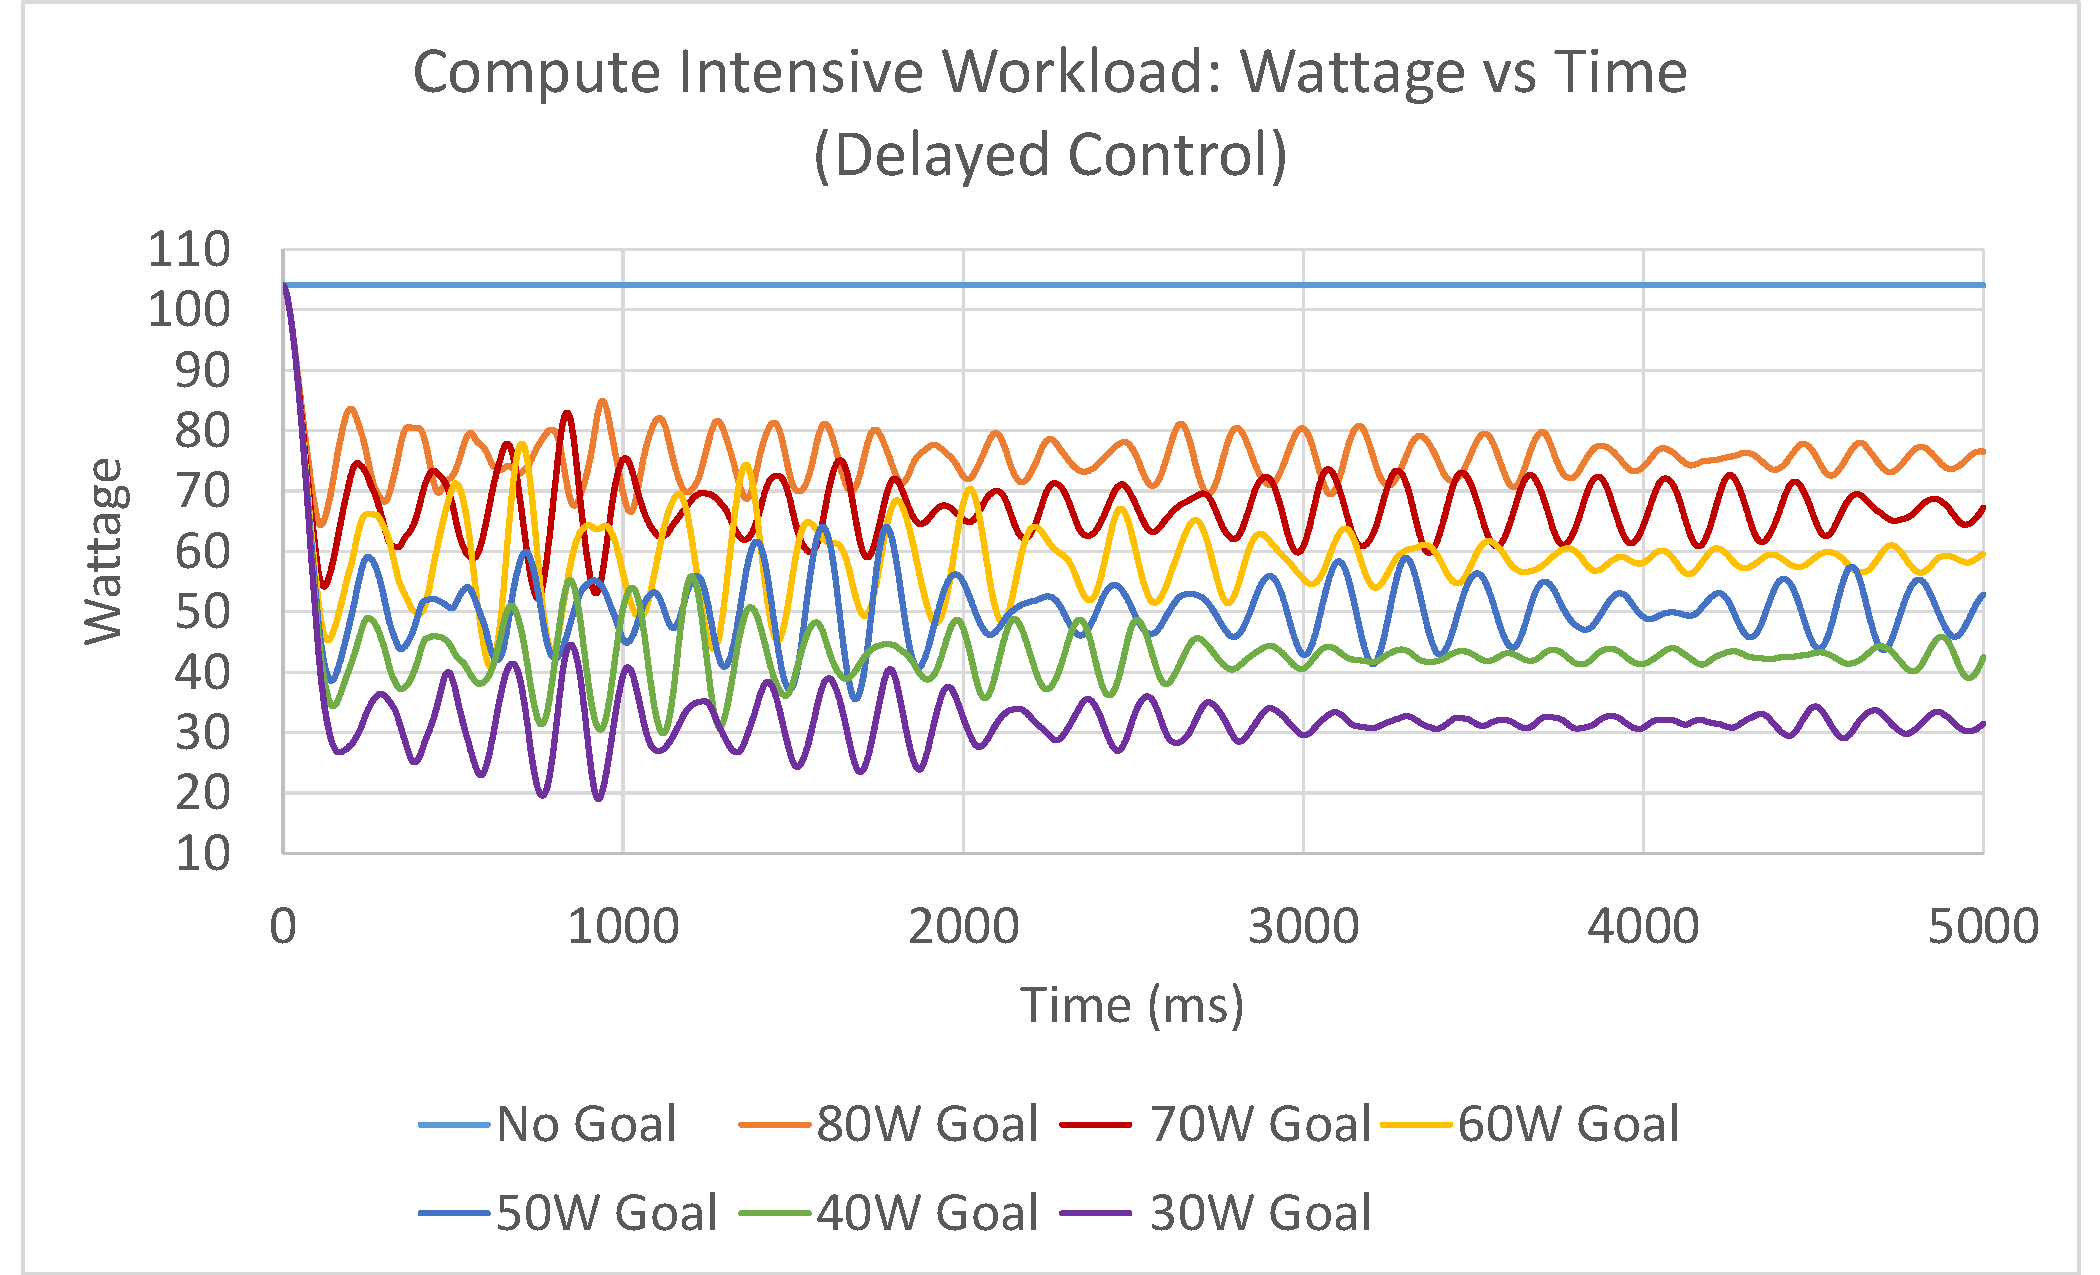
\includegraphics[width=0.82\textwidth]{Fig/compute_delay_graph.pdf}
                \caption[Compute Intensive Workload Using an Adaptive Goal Adjustment Policy with Differing Delayed Control (Watts vs Time)]{Shown is the result of over damping a distributed control policy to adaptively reach a target goal for a stable compute intensive load.}
                \label{fig:compute_delay_graph}
            \end{figure}

            One way in which a distributed hierarchical adaptive system can cause maladaptive behavior is by not quickly enough adapting to state changes. This will result in unpredictable oscillations as shown in figure~\ref{fig:compute_delay_graph}. In a localized adaptive scheme, one might see predictable oscillations if miscalibration of this manner were to occur, but in a distributed system the behavior is more complicated and more difficult to diagnose. The key reason for the unpredictable oscillations is that as the control hierarchy operates independently, control engines will attempt to converge independently of one another leading to differing levels of over compensation at differing points of time.

            In a real system, this behavior could be the result of incorrect information being aggregated up the control hierarchy, information not being passed quickly enough to higher level control engines, the result of control decisions taking too long, or the result of delay in sending control decisions to lower level control engines. It is for this reason that a complicated decision making process involving long computations will not be possible in an massively distributed control engine hierarchy. Decisions must be quick and correct in real time in order to compensate for execution behavior. While offline learning could be used to improve the behavior of adaptive policies, the online components must be calibrated and responsive in terms of (1) receiving up-to-date information, (2) making adaptive decisions, and (3) sending those adaptive decisions down the hierarchy.

            \begin{figure}[htb!]
                \centering
                \includegraphics[width=0.82\textwidth]{Fig/compute_no_delay_graph.pdf}
                \caption[Compute Intensive Workload Using an Adaptive Goal Adjustment Policy with Under Damped Control (Watts vs Time)]{Shown is the result of under damping a distributed control policy to adaptively reach a target goal for a stable compute intensive load.}
                \label{fig:compute_no_delay_graph}
            \end{figure}

            Another way in which a distributed hierarchical adaptive system can cause maladaptive behavior is by making decisions too quickly or not giving enough time for prior decisions to take effect. This will result in predictable patterns as shown in figure~\ref{fig:compute_no_delay_graph}. The characteristic saw tooth pattern seen in the figure is the result of a limit cap on increased power changes over a given time period for the particular policy. In a localized adaptive scheme, an under damped system will result in similarly predictable oscillations depending on the exact policy. In this particular case, only the higher level control engines are over damped, meaning that if the lower level layers of the system were left alone with set goals they would converge to them. However, when the upper level layers of the hierarchy are maladaptive the effects sweep across the system making it unable to effectively adapt.

            In a real system, this behavior could be the result of simply miscalibrated control engines. Another way this might occur is in the event that decisions take a long time to take effect. For example, if a decision is made to power gate a core or block of a real system, it is possible that a delay could occur and that new aggregated data information being sent will not include the effect for some time. A hierarchical decision process needs to be aware of delays in the control knobs that exist in the system in order to effectively adapt. Additionally, predictive proactive policies that account for time delay may be needed to actively adapt if the delay is large. 

            \begin{figure}[htb!]
                \centering
                \includegraphics[width=0.82\textwidth]{Fig/compute_differing_graph.pdf}
                \caption[Compute Intensive Workload Using an Adaptive Goal Adjustment Policy with Differing Rates (Watts vs Time)]{Shown is the result of varying damping rates within a given level in a distributed control policy to adaptively reach a target for a stable compute intensive workload.}
                \label{fig:compute_differing_graph}
            \end{figure}

            A third way in which a distributed adaptive control system can go awry is by differing the control rates of control engines in a maladaptive manner. This behavior is shown in figure~\ref{fig:compute_differing_graph}. This demonstrates that even slightly miscalibrated controllers can cause rippling oscillations throughout the system instead of convergence toward a goal in the presence of a stable workload. While the effect demonstrated is not that bad under stable conditions, it may certainly result in unpredictable behavior in unstable workloads. This highlights the critical need for distributed control systems to be able to identity maladaptive components and mitigate their effects.

            In a real system, this behavior would most likely be the result of simply miscalibrated control engines and only lead to small effects. It is worth noting that such behavior could cause emergent maladaptive behavior that is not detectable within a stable isolated workload. As we will demonstrate with other workloads, maladaptive behavior can cause much worse oscillations within an adaptive system. As such, real systems should provide mechanisms to identity maladaptive components either online or offline in order to provide systems engineers with a clear methodology to fix such issues, as well as, for system software to adapt in the presence of unstable system components.
        %}
    %}
    \subsection{Network Intensive Workload}
    %{
        This section demonstrates effective adaptive policies that generally converge toward a solution for a network intensive goal once given a goal. Additionally, adaptive behavior in the presence of maladaptive components is discussed in detail.

        \subsubsection{Adaptive Solutions}
        %{
            \begin{figure}[htb!]
                \centering
                \includegraphics[width=0.82\textwidth]{Fig/network_goal_adjustment.pdf}
                \caption[Network Intensive Workload Using an Adaptive Goal Adjustment Policy (Watts vs Time)]{Shown is the effect of an adaptive control policy that lowers and raises sub-control engine goals when its goal is not met for a network intensive workload. It is capable of meeting its goal; however, undershoots in some cases possibility due to overcompensating localized control engines.}
                \label{fig:network_goal_adjustment}
            \end{figure}
    
            The experiments discussed in this section show the ability of a hierarchical adaptive system to adapt to a network intensive workload. The two policies used are the adaptive goal adjustment and benefit policies discussed in section~\ref{sec:policies}. These two policies are designed to make minimal adjustments when near a goal and to let lower level control engines converge to a solution with minimal interference when lower level control engines are doing their job effectively. These higher level policies show good behavior both when lower level policies are doing their job and when they aren't. The subsequently discussed experiments show the former case.

            \begin{figure}[htb!]
                \centering
                \includegraphics[width=0.82\textwidth]{Fig/network_benefit.pdf}
                \caption[Network Intensive Workload Using a Benefit Policy (Watts vs Time)]{Shown is the effect of an adaptive control policy that attempts to intelligently reduce slack in load by raising the goal of lower control engines when others fall below their goals. Essentially, it reduces the goal of engines currently below their goal, and increases the goal of other engines.}
                \label{fig:network_benefit}
            \end{figure}

            Figures~\ref{fig:network_goal_adjustment} and~\ref{fig:network_benefit} demonstrate the ability of these policies to converge to a stable solution. The benefit policy is better able to converge to the overall system goal; whereas, the random goal adjustment policy undershoots in some cases. Though, these experiments demonstrate that hierarchical adaptive controls work well during stable network phases, more importantly, the goal adjustment policy is demonstrated to effectively adapt under unstable maladaptive conditions in Section~\ref{sec:network_maladaptive_behaviors} and under phased workloads in Section~\ref{sec:phased}. 
        %}

        \subsubsection{Maladaptive Behaviors}
        %{
            \label{sec:network_maladaptive_behaviors}
            The experiments discussed in this section highlight how limited granularity of control mechanisms can lead to maladaptive behavior, as well as, the effect maladaptive components can have on convergence toward a goal. They also serve to demonstrate how hierarchical control can mitigate some of the effects of maladaptive components.

            \begin{figure}[htb!]
                \centering
                \includegraphics[width=0.82\textwidth]{Fig/network_coarse.pdf}
                \caption[Network Intensive Workload Using an Adaptive Goal Adjustment Policy with Coarse-grain Control (Watts vs Time)]{Shown is the result of providing only coarse grain adaptive network controls to lower level control engines. Network activity is capped to a minimum of 50\% for a network intensive workload.}
                \label{fig:network_coarse}
            \end{figure}

            If controls are too coarse-grained this can lead to the inability to effectively adapt for any control system. Figure~\ref{fig:network_coarse} shows an example of the effects that might occur in such cases. Shown is a network control mechanism that is limited to 50\% of the maximum rate. By capping the limit, the effective minimum wattage of a network intensive workload is around 60 watts because the lowest level control engines can do nothing else to limit activity under the policy. If one were to limit activity to large percentage, 5\% for example, these engines would similarly be unable to meet a goal and would simply oscillate around the goal never converging. While in some sense, this is a unnatural example, it serves to highlight an important point about the granularity of adaptive mechanisms. For example, a real system with hard limits on the granularity of core DVFS states might similarly be unable to meet goals. Instead, cores may oscillate around a goal. As such, the granularity of controls will be a critical aspect in exascale systems.

            \begin{figure}[htb!]
                \centering
                \includegraphics[width=0.82\textwidth]{Fig/network_maladaptive.pdf}
                \caption[Network Intensive Workload Using an Adaptive Goal Adjustment Policy with Maladaptive System Components (Watts vs Time)]{Shown is the result of introducing 64 maladaptive lower level control engines under an adaptive control policy for a network intensive workload. Essentially, the working control engines have mitigated the effects of these other malicious components when possible. In cases such as this, higher level control engines revaluate and assign goals accordingly.}
                \label{fig:network_maladaptive}
            \end{figure}

            Given a distributed system, components may be maladaptive in some way. That is to say, unable to meet a goal for some reason. For example, as discussed above, coarse-grain controls may lead localized control engines to be unable to directly meet a goal. However, in the event of a maladaptive component within the system, a distributed control hierarchy should be resilient enough to detect maladaptive components and minimize the effects; and to meet their own goal if possible. Shown in Figure~\ref{fig:network_maladaptive} is a hierarchical adaptive policy's ability to cope in the event that $\frac{1}{4}$ of components within the system ignore commands and continue operating at maximum frequency and network state. While the system cannot meet a goal below 40 watts, it is perfectly able to converge to a solution for higher goals. This serves as testament to the ability of distributed control engines to cope with maladaption. Local static control policies would simply be unable to cope with such behavior. This is explored in more detail in Section~\ref{sec:phased}.
        %}

    \subsection{Phased Workload}
    %{
        \label{sec:phased}
        This section is devoted to discussion of hierarchical and local adaptation schemes under phased workloads. The particular phased workload, and conditions under which it is run, is designed to stress adaptive schemes, such that, they have a very difficult time converging to an acceptable solution. The central idea is to operate these adaptive schemes under the worst conditions and to demonstrate their effectiveness or non-effectiveness.
        
        \subsubsection{Adaptive Solutions}
        %{
            This section demonstrates effective adaptive solutions for the phased workload. Both wattage and temperature levels for the adaptive goal adjustment policy are shown. As will be denoted below, wattage goals directly translate into temperature goals. The duality of the two is an important aspect not to be understated. 
 
            \begin{figure}[htb!]
                \centering
                \includegraphics[width=0.82\textwidth]{Fig/phase_hier.pdf}
                \caption[Phased Workload Using an Adaptive Goal Adjustment Policy (Watts vs Time)]{Shown is a hierarchical adaptation scheme adapting to a phased workload of local and network operations. Demonstrated is that hierarchical adaptation schemes are capable of effectively mitigating and managing the effects of over and under compensating local control engines.}
                \label{fig:phase_hier}
            \end{figure}

            Figure~\ref{fig:phase_hier} demonstrates that even for highly oscillating workloads consisting of quickly varying phases, hierarchical adaptive schemes are effective and converge to their goal even in the event of a 70 Watt swing at full operation. In this particular case, we see an initial drop in wattage as the scheme takes effect and then a rise and quick convergence. The reason for this behavior is that the policy used immediately drops network activity to a minimum if it is causing control engines to miss their goal by a large amount. As will be demonstrated with subsequent experiments, complete convergence is not possible with static localized schemes and under conditions with maladaptive components, no localized adaptive solution is possible.
            
            \begin{figure}[htb!]
                \centering
                \includegraphics[width=0.82\textwidth]{Fig/phase_hier_temp.pdf}
                \caption[Phased Workload Using an Adaptive Goal Adjustment Policy (Temperature vs Time)]{Shown is a hierarchical adaptation scheme adapting to a phased workload of local and network operations. Demonstrated is that hierarchical adaptation schemes are capable of meeting temperature goals indirectly through wattage goals.}
                \label{fig:phase_hier_temp}
            \end{figure}
            
            Figure~\ref{fig:phase_hier_temp} shows the same phased workload collecting average temperature instead of wattage. It demonstrates that wattage goals necessarily translate into temperature goals. This is due to the nature of average chip temperature levels being the direct result of wattage levels. A hierarchical scheme capable of meeting wattage goals will necessarily be able to meet temperature goals as well. In fact, because temperature changes more slowly than wattage levels, it is easier to for an adaptive scheme to meet temperature goals on average. This is evident when comparing Figure~\ref{fig:phase_hier} to Figure~\ref{fig:phase_hier_temp} where it is shown that temperature levels converge more quickly than wattage and have less variation over time. As such, it is reasonable to expect wattage goals to be used in conjunction with chip specifications to meet a temperature goal instead of directly using temperature goals and temperature machine specific registers. However, this does not preclude using temperature goals directly if so desired. A policy capable of meeting wattage goals within SAFE would need only to collect temperature averages instead of wattage and adapt on those directly. In fact, the aggregation of temperature data is already implemented, but the adaptive policies within SAFE simply use wattage instead. The purpose here is to simply demonstrate that there is a duality between wattage and temperature and that meeting one goal necessarily means meeting the other. Of course, in reality, absolute temperature junction thresholds should always be met. That is to say, if a chip cannot operate above a certain temperature, then built in safe guards should be in place to ensure that it never goes above that temperature outside of higher level system software adaptive schemes. One would expect such a mechanism to be implemented in low level firmware. 
        %}

        \subsubsection{Maladaptive Behaviors}
        %{
            This section demonstrates the effectiveness of hierarchical adaptation under maladaptive conditions, as well as, the behavior of localized adaptation schemes under non-optimal conditions. As will be shown, localized adaptive schemes perform poorly in the presence of maladaptive behavior. 

            \begin{figure}[htb!]
                \centering
                \includegraphics[width=0.82\textwidth]{Fig/phase_local.pdf}
                \caption[Phased Workload Using a Greedy Local Only Adaptive Policy]{Shown is the result of using a localized adaptation scheme with preset goals for adapting a phased workload of local and network operations. Oscillation is present for all goals and convergence toward a stable solution is not guaranteed.}
                \label{fig:phase_local}
            \end{figure}

            Figure~\ref{fig:phase_local} shows the behavior of the phased workload under a statically allocated local adaptive policy. Essentially, what we see is that minor overcompensation by individual control engines leads to oscillations within the system. This reason for this behavior is that though individual overcompensations by themselves are minor, accumulated together, they result in a large wattage swing all at once. Localized adaption schemes cannot mitigate this behavior because they do not have an idea about the current overall wattage state of the system. 

            \begin{figure}[htb!]
                \centering
                \includegraphics[width=0.82\textwidth]{Fig/phase_zoom.pdf}
                \caption[Phased Workload Local Only vs Hierarchal Adaptation (Watts vs Time)]{Shown is a close up view of a local adaptive policy against a hierarchical policy in adapting to a phased workload.}
                \label{fig:phase_zoom}
            \end{figure}

            Figure~\ref{fig:phase_zoom} demonstrates this more clearly by plotting the localized adaptation scheme against the hierarchical scheme discussed above. For a localized adaptive scheme, there are consistently 10 watt swings as the system over and under compensates repeatedly. Where as, the hierarchical adaptive scheme detects and mitigates the trend through the aggregation of data at higher levels of the control hierarchy. Essentially, higher level engines see the large trend that localized schemes are incapable of detecting. This is an important adaptive behavior the spans not only power, but also temperature, or any other system goal. When combined with thousands of individual cores, maladaptive localized behaviors such as these will become a significant problem. The subsequent experiments introducing maladaptive behavior into the control system will demonstrate this even more profoundly.

            \begin{figure}[htb!]
                \centering
                \includegraphics[width=0.82\textwidth]{Fig/phase_local_maladaptive.pdf}
                \caption[Phased Workload Using a Greedy Local Only Adaptive Policy with Maladaptive System Components (Watts vs Time)]{Shown is the result of using a localized adaptation scheme with preset goals for adapting a phased workload of local and network operations in the presence of 64 maladaptive control engines. Extensive oscillation is present for all goals and convergence is not possible due to the nature of localized adaptive schemes to not account for the behavior of other components within a system.}
                \label{fig:phase_local_maladaptive}
            \end{figure}

            \begin{figure}[htb!]
                \centering
                \includegraphics[width=0.82\textwidth]{Fig/phase_hier_maladaptive.pdf}
                \caption[Phased Workload Using an Adaptive Goal Adjustment Policy with Maladaptive System Components (Watts vs Time)]{Shown is a hierarchical adaptation scheme adapting to a phased workload of local and network operations in the presence of 64 maladaptive control engines. Despite an extensive amount of maladaptive components within the system, the control hierarchy does a good job mitigating the effects and demonstrates the resiliency of hierarchical solutions. Convergence toward a solution would be impossible under such conditions with a localized adaptive scheme.}
                \label{fig:phase_hier_maladaptive}
            \end{figure}

            \begin{figure}[htb!]
                \centering
                \includegraphics[width=0.82\textwidth]{Fig/phase_zoom_maladaptive.pdf}
                \caption[Phased Workload Local Only vs Hierarchal Adaptation with Maladaptive System Components (Watts vs Time)]{Shown is a close up view of a local adaptive policy against a hierarchical policy in adapting to a phased workload in the presence of maladaptive system components.}
                \label{fig:phase_zoom_maladaptive}
            \end{figure}

            Figure~\ref{fig:phase_local_maladaptive} shows the same localized adaptation scheme for the phased workload in the presence of $\frac{1}{4}$ of the system exhibiting maladaptive behavior. In this particular case, not only is the system not able to converge to a goal, the localized adaptation scheme results in very large oscillations on the order approximately 40 watts. This behavior is not surprising given that a localized scheme means that well behaved control engines only know about the behavior of components under their control and not other maladaptive sections of the system. But, it highlights an important aspect of adaptive policies within massively scale systems. That is to say, maladaptive components will cause systems to be unable to meet goals without hierarchical adaptive schemes in place.
            
            If we take a look at Figure~\ref{fig:phase_hier_maladaptive}, it shows that even in the presence of large oscillations that result from the maladaptive components, that the hierarchical distributed adaptive schemes perform extremely well considering the conditions under which it is operating. This is shown more clearly in Figure~\ref{fig:phase_zoom_maladaptive} comparing the localized adaptive scheme to the hierarchical adaptive scheme. In one case, the goal is met following small oscillations to convergence and in the other case the goal never met.
    
            In essence, this shows the effectiveness of hierarchical adaptive solutions and makes an argument for the usage of these types of solutions in systems operating at this scale. Demonstrably, localized static schemes will certainly not suffice in cases such as this. With the variability in the operating states of individual cores due to yield, these types of behavior are set to become more common in exascale hardware. Even in cases where the hardware works appropriately, localized maxima and minimas could result in behaviors such as this due to workload patterns or non-optimal localized adaptive engines. Additionally, optimized workloads will certainly result in hot spotting in terms of system resource utilization not shown in these experiments. Static allocation of resources would result in non-optimal solutions not only affecting the wattage as shown here, but also the performance of executing workloads. Ideal adaptive solutions would allocate wattage where needed while converging toward overall system goals.
        %}
    %}
    \subsection{Overall Discussion}
    %{
        Overall, the experimental results demonstrate the need for hierarchical adaptive policies in exascale architectures. Even for relatively stable non-phased workloads, problems meeting goals will occur if individual components are unable to meet their local goal and no higher level adaptive policies are in place to mitigate the effects. In cases with phased workloads, the effects will result in unpredictable behavior due to localized oscillation in different sections of the chip. In conjunction with high levels of maladaptive behavior, this can result in a very large deviation from the specified goal. On other hand, hierarchical adaptive policies are capable of significantly mitigating the effect of maladaptive behavior. Additionally, hierarchical adaptive schemes perform better even when all sections of the system are behaving appropriately in comparison to localized schemes. As discussed earlier in this chapter, this is primarily due to the higher level adaptive engines having a more complete picture of system behavior; and thus, being able correct the overcompensation of localized adaptive engines.

        It is important not to understate the need to maintain a particular granularity of control in terms of adjustable system knobs. As was shown in experimental results, coarse-grain control can lead to an inability for the lower level control engines to meet localized goals. This could simply be the result of an inability to turn off enough components to lower power or temperature to a desired level, or it could be the result of knobs not having enough levels and simply causing oscillations above and below the localized goal. An example of this would be a control engine only capable of switching off an entire block of execution engines at once (8 XEs within SAFE). While higher level adaptive schemes will no doubt mitigate the bad effects of this behavior, the lower level engines may never converge to a solution (depending on their workload); thus causing, jitter and a higher convergence time for higher level system goals.
    %}
%}
    \chapter{Related Work}
        \label{chap:related_work}
This chapter discusses prior related work in self-adaptation and self-awareness to give the reader a brief understanding of the many different aspects of adaptation. Approaches range from designing adaptive hardware to cross-layer techniques that focus on using hardware and software together to build adaptive systems or applications. Many approaches focus on specific applications or subclasses of application and as such do not consider any notion of system level adaptation which is of an integral importance within exascale systems. Other approaches focus on providing some type adaptation for specific components within a system and could be incorporated into exascale hardware or even exposed to system software. Research into system level adaptation is generally in the form operating systems or management of resources. Newer bodies of work attempt to treat adaptation more holistically, and provide solutions that span multiple layers of the system from hardware to the high-level software.

For the purposes of this discussion, we group different approaches to adaptation into four categories: Application Centric Adaptation, Component Centric Adaptation, System Centric Adaptation, and Cross-layer Adaptation. {\it Application Centric Adaptation} focuses on adaptation within specific applications using either hardware or software techniques. {\it Component Centric Adaptation} focuses on monitoring or adaptation within a particular component or resource of a system. {\it System Centric Adaptation} focuses on adaptation at the system level. {\it Cross-layer Adaptation} focuses on adaptation across multiple layers of the system software stack. Following this, we discuss the aspect of predictive system modeling. Finally, we discuss state of the art self-adaptive frameworks and the features they exhibit and the aspects of exascale adaptation that make it fundamentally different from prior research.

\section{Application Centric Adaptation}
%{
    Application centric approaches focus on adaption for specific applications or a subclass of applications within a given domain. Because this type of adaptation is largely not generalizable outside of specific applications; and thus, incompatible with our goal of a general self-aware system, we mention these only in passing for completeness sake.
    
    Quality of service (QoS) is one large area of active research~\cite{AbdelzaherShin1998, CardelliniEtAl2012, IvanovicEtAl2010, LuEtAl2006, ZhengEtAl2010} due to the real time requirements and the ever changing field of computing resources. Many newer works focus on cloud computing in particular~\cite{KumarEtAl2013, WangEtAl2013}. Other works focus on changing application specific algorithm policy~\cite{ThomasEtAl2005}.
    
    Some approaches are more akin to toolkits designed for application programmers to use to enable adaptation within their software~\cite{GoelEtAl1998, GoelEtAl1999}. Many of these approaches listed incorporate some form of classical control theory because of various provable guarantees such as stability and linearity, etc.; however, in more recent years, there has also been a shift toward heuristic based tuning and machine learning techniques~\cite{MaggioEtAl2011} because, though not providing the provable guarantees of classical control theory, these tend to provide more robust adaptivity in practice with real applications.
%}
\section{Component Centric Adaptation}
%{
    Component centric approaches are a form of adaptation that focuses on monitoring and adapting a particular components or resources of a system. These can include such facets as networking, memory, and cache, among other things. Many of these works focus on introducing dynamic reconfigurability into the hardware or at the software level. There is much work to be found along these lines but for brevities sake we focus on only a few newer works.
    
    Some work focuses on introducing adaptive reconfigurability into memory organization. One such work~\cite{SaM_2013} proposes a self-aware memory (SaM) which includes a self-optimization process. The memory itself is partitioned into self-managing components and dynamic memory allocation is done using a client-server style technique to reduce bottlenecks. In order to optimize memory allocation, each memory component has knowledge of allocated blocks, access rate, and ownership, as well as, limited knowledge of the state of neighboring memory components. An extended memory management unit (MMU) is responsible for memory requests and uses acquired knowledge to to optimize memory allocations. Another work~\cite{IpekEtAl2008} proposes a self-optimizing memory controller that operates using the principles of reinforcement learning (RL). It works by formulating the scheduling of data reads and writes as a reward based structure. If a command leads to data bus utilization, this is marked as a reward of one; otherwise, zero. Using accrued data in conjunction with the controller's state (number of reads, writes, and misses, etc.), the controller can learn to optimize various aspects of its operation, such as, balancing reads and writes, detect states that lead to low levels of requests and avoid those in advanced by prioritizing load misses, amortize write-to-read delays, etc.
    
    Other work focuses on introducing hardware reconfigurability into the caching aspects of memory. One such work~\cite{Balasubramonian2000,BalasubramonianEtAl2000} proposes incorporating dynamic reconfiguration into the caching levels of memory hierarchies. In essence, the hardware is capable of detecting phase changes in the access pattern of applications to react to hit and miss intolerance by adjusting the hierarchy from a three-level cache to a two-level cache and vice versa. Another work~\cite{WangMishra2009} proposes dynamically adjusting the associativity and line sizes using similar techniques. Still other works~\cite{KimEtAl2002} focus on the non-uniform cache access (NUCA) times associated with large multi-megabyte caches and propose logical policies to allow data to migrate adaptively to memory banks with less cycle access times for given processors depending on the access pattern.
    
    There are a number of works that focus on introducing adaptive reconfigurability into networks or network interfaces. One such work~\cite{NoC_2013, NoC_2014} develops a network-on-chip (NoC) with dynamically configurable memory buffers (FIFO depth) and a dynamically configurable time division multiple access (TDMA) scheduler which can adapt the number of time slots for different communications according to measured bandwidth. Hardware mechanisms are incorporated to expand and shrink FIFOs depending on utilization. Additionally, genetic algorithms are used to optimize TDMA table access. There has been additional work done on tackling network adaptation at the software level. One such work~\cite{Gelenbe2013} focuses on retaining past QoS performance information for given hops along destination from source to enable the source to make better decisions about the path to send packets along in the future.
%}

\section{System Centric Adaptation}
%{
    \label{sec:SystemCentric}
    System centric approaches focus on adaptation at the system level. These are software level approaches that tend to use existing hardware and the operating system (OS) for adaption. Historically the role of resource management has been given to the operating system. In the case of highly parallel systems, we can divide these approaches into several categories: full OSes, lightweight kernels, micro kernels, and high-level runtime systems.

    \subsection{Full OSes}
    %{
        High-performance systems which use so-called Full OSes take advantage of off-the-shelf systems, and tune them to reduce system noise. Such approaches are often embodied in cluster-like environments~\cite{SterlingEtAl95}. Even on dedicated supercomputers, these approaches have been followed, as they provide a programming environment which allows for maximal flexibility. However, such systems are in general ill-prepared for the requirements of future extreme-scale/exascale high-performance environments: their control over the power envelope is only at a very coarse-granularity; resilience is left to third party systems, and is not considered as part of the whole; they are oblivious of the needs of the application they host; etc. Finally, full OSes leave very little room for specialization.
    %}

    \subsection{Light-Weight Kernels}
    %{
        Another approach is to rely on so-called light-weight kernels or LWKs~\cite{GiampapaEtAl10, BallesterosEtAl12}. LWKs offer many advantages over full OSes: They are usually written from scratch, and only re-implement features needed for an HPC environment. The source code being much smaller, means bugs are easier to track and fix. Finally, being specialized kernels, they usually emit very little noise when running an application on top of LWKs. They also do expose significant limitations: they very often require the user to learn a new API to communicate with the system; if a feature usually provided by full OSes is missing from the LWK, the user's application may not be portable to the system. In general, the application programmer does require features found in traditional OSes. Some LWKs do forward calls to ``missing'' features to a  ``heavier'' kernel however. %\textbf{[TODO: \\cite]}
    %}

    \subsection{Micro-Kernels}
    %{
        Micro-kernels strip down OSes to the bare minimum (i.e. address space management, process/thread management, inter-process communication). These so called kernels run in privileged mode (e.g. ring0 on x86 architectures), while providing satellite features which enrich the overall system, but in an unprivileged mode (for example, a file system driver). Micro-kernel OSes have shown they could be robust and thus fulfill the resiliency and maybe even the power and energy requirements (as only the required services are running). However, for many years, performance was lacking, due to the message-driven orientation of most implementations. 

        New approaches have tried to revive micro-kernels, as well as, remove the layers that historically introduced overhead~\cite{AppavooEtAl05,KriegerEtAl06,NightingaleEtAl09,SachaEtAl12}. Indeed, message-driven communication in micro-kernels tend to suit multi- and many-core systems very well. However, there is no approach that tries to provide a holistic view of performance, power, and resiliency for different granularities. However the latest efforts around micro-kernels have evolved toward a more library-oriented approach for operating systems~\cite{AmmonsEtAl07}. Such approaches tend to have goals that are closer to our own.
    %}

    \subsection{High-level Runtime Systems}
    %{
        High-level runtime systems typically implement some form of resource management on top of an existing OS. Typically they intend to provide some type of policy management that doesn't exist in the underlying OS. Some focus on providing QoS of system resource~\cite{LiNahrstedt2001, LiEtAl2006, Sharifi2011} or provide resource management with dynamic policies~\cite{ZhangEtAl2002}. Others are in the form of languages or frameworks that provide mechanism for an application to adapt~\cite{ChangKaramcheti2000, HollingsworthEtAl1998, RiblerEtAl1998, SironiEtAl2012}.
    %}
%}

\section{Cross-layer Adaptation}
%{
    Cross-layer approaches involve implementing introspective capabilities across multiple levels of the system software stack. These differ from the system level approaches discussed in section~\ref{sec:SystemCentric} in that they are designed specifically to expose capabilities to differing levels of the software stack; whereas, system centric approaches tend to keep most control at the operating system level. For example, these approaches may place monitoring capabilities at the OS kernel level and adaptive capabilities at the application level. These types of approaches served as inspiration for the work contained within this thesis.
    
    The SElf-awareE Computing (SEEC) model~\cite{Hoffmann2010,Hoffmann2012,Hoffman2013} by Hank Hoffman in many ways is the father of self-aware computing, as well as, father of cross-layer approaches to adaptation. It incorporates an observe-decide-act feedback loop with, at its core the notion of expressing goals as application heartbeats. In essence, using a HeartBeat API, an application registers heartbeats at some specified interval as well as a target heart rate to reach. Additionally, a precision goal can be registered (e.g. maximize performance at some user defined peak-signal-to-noise ratio - PSNR). In the background, SEEC observes the heart rate and the controller calculates the adjustments needed at the next time step. Offline, a series of actuators, possible states, and the costs/benefits of those states are defined. The cost/benefits associated with each actuator are used in the decision making process to determine the best course of action in the next time step. SEEC then applies actions by adjusting actuators to the appropriate state. Actuators can either be system level (e.g. core frequency) or application specific (e.g. which video codec to use). Additionally, reinforcement learning is used to adjust the costs/benefits of each actuator, thus enabling the system to eventually converge to meet the demands of the target heart rate. Video decoding is an often seen example application used with SEEC. In this particular case, frames-per-second (FPS) can easily be expressed as a target heart rate. After each frame is rendered the application registers a heart beat and SEEC keeps track of the heart rate (FPS). If the current heart rate is either lower or higher than than the target heart rate then SEEC will adjust a number of different actuators until the heart rate is met. In this particular case, various decoding parameters can be adjusted on the fly as well as system specific actuators. Because the actuators affect the quality of rendered images, a PSNR goal can be used to ensure that the output quality does not become too low. Similarly, power goals can be specified to allow for the application to reach a target heart rate while minimizing power usage. The generalized controller design and cross-layer nature of SEEC has shown promising results when used in conjunction with specialized hardware features. One such work combines SEEC with a processor that incorporates energy monitoring circuits~\cite{SinangilEtAl2014} to augment SEEC's energy adaptation capabilities.
    
    Another work, CoAdapt~\cite{Hoffmann2014}, also by Hoffman, seeks to alleviate some of the shortcomings of the prior work. While SEEC could only provide guarantees for a single dimensional goal in terms of power or performance, or accuracy; CoAdapt, can provide guarantees for two out of the three dimensions while also optimizing the third. CoAdapt segments goal dimensions such that one is the lead and the other is the subordinate. The overall configuration of the lead dimension is used to predict how the primary goal will affect the subordinate dimension and the system uses this information to dynamically adapt and ensure the latter dimension doesn't oscillate and instead converges to its goal.
    
    Some approaches focus on runtime level adaptation using information from lower levels of the software stack. A work, by Gioiosa~\cite{GioiosaEtAl2014}, applies classical control theoretic techniques to implement adaptive behavior across the software stack using a self-feedback control loop. At the kernel level, a kernel module based monitor observes current system values and compares those to reference values in order to apply self-correction. A controller, implemented at the runtime level (e.g. OpenMP, etc.), communicates with the monitor to make adjustments, such as, adjusting the number of process threads. A well defined communication interface is used to facilitate the sending and receiving of information and commands between the components. The primary focus of the work is on decoupling the low-level details of the system (from a monitoring sense) from high-level programming models or runtimes which want to incorporate adaptive decision making.
%}

\section{Modeling}
%{
    A number of works focus primarily on the aspect of predictive modeling of system behavior. Though these works do not necessarily implement a cross-layer adaptive approach, they are an integral piece in an adaptive solution that could be used in any layer of a software stack from application level to runtime level. For this reason, we discuss these works here. It is worth noting that these types of work do not conflict with work found in this thesis, and indeed, we expect modeling to be an important aspect of the predictive capabilities of future exascale systems.
    
    One work develops a power model based on PMU information and extends linear and neural network models to account for external temperatures to build an adaptive predictive power modeling solution for existing hardware~\cite{AhmadEtAl2015}. The model separates events into three categories: (1) local within a core, (2) events occurring within shared resources, and (3) events available at the OS level. Algorithmic models are used to adaptively choose relevant events for modeling while discarding irrelevant events for performance overhead reasons. The novelty of the approach is that the interactions of events is considered during the selection process. The selection process uses a data mining inspired sub-space method to greedily search for the best events using Correlation Feature Selection~\cite{HallHolmes2003}. For power modeling, a linear approximation of traditional RC circuits is used.
%}

\section{Discussion}
%{
    \label{sec:related_work_discussion}
    This section is devoted to discussion of the important aspects toward developing a truly self-aware exascale system. Let us begin by discussing the numerous challenges of exascale and then following this by a discussion of the general limitations in current bodies of research. Some of the important challenges of exascale include the management of power and energy~\cite{Dally2011}, as well as, performance across hundreds to thousands of cores. Furthermore, these seemingly conflicting goals cannot be considered in isolation. A coordination between system resources, components, and applications will be integral at the exascale level to coordinate and adapt.

    In terms of exascale applicability, application level approaches to adaptation focus far too narrow in scope on specific applications and lack a holistic view. These tend to lack an appreciation for the system level challenges discussed above, and in many cases could directly conflict with or hinder cross-layer adaptive goals, such as, minimizing energy expenditure. That is not to say that application goals should not be considered in an exascale system. In fact, applications will need to become first class citizens in the sense that their goals will need to be accounted for by a self-adapting system. However, application goals should be expressed in the form of hints to system level software given that such software will have better and more complete information to make scheduling and other decisions upon.
    
    For exascale adaptivity, component level adaptation does not necessarily hinder a cross-layer approach to adaptation. Indeed, if the right interfaces were exposed within the hardware, it could very well aid a cross-layer approach to adaptation. And software level component adaptation (such as software QoS) could be incorporated directly into cross-layer approaches. For the most part, these types of approaches are neither here nor there with respect to the work discussed in this thesis; however, we do take inspiration from these in terms of exposing hardware features or creating software features that allow cross-layer adaptation of specific hardware components.
    
    Research into system level adaptation, as discussed previously, is generally in the form of operating systems or in the management of resources. However, these approaches lack fine-grained control over hardware components due to limitations in hardware. Exascale architectures will need to adjust the state of components at a very fine granularity in order to conserve energy and to meet power envelopes. This is one important area where exascale research breaks from the current state of the art in that a co-design of hardware and software will yield a system that is capable of adapting in ways not possible in current generation systems. As such, outside of limited research, system software design has not generally attempted to conquer the challenges of exascale. Moreover, there is a large change in scope both in terms of hardware heterogeneity and the vast expansion in the number of components that will need to be taken into account for adaptation. As previously mentioned, there is also an expansion in the goals and types of adaptation that need to occur in exascale systems.
    
    The current trend in adaptive computing has been to focus on energy adaptation in some form~\cite{BaekEtAl2010, SorberEtAl2007} as this is integral for low power domains and now increasingly for exascale architectures. SEEC, one of the seminal works in self-aware computing,~\cite{Hoffman2013} focused on both energy and performance adaptation using a notion of ``application heartbeats.'' These allowed for an application to communicate goals to a system as well as progress toward those goals. The results showed that various applications could be instrumented with heart beats and capable of adapting to meet both energy and performance goals. However, SEEC relied heavily on application instrumentation and thus is arguably limited to applications that fit a certain paradigm. Additionally, it supported only application goals; as opposed to more more general system level goals. It also relied on the programmer to understand and provide a notion of progress toward a goal; which may not be possible in all applications. Finally, it lacked support for handling conflicting goals or more generally multi-variable problems. CoAdapt~\cite{Hoffmann2014} sought to eliminate some of these shortcomings by providing limited support for adapting to multiple conflicting goals; however, many of the other challenges and limitations mentioned above were not addressed. Other cross-layer approaches while focusing on exposing hardware monitoring to runtime level software tend to focus on existing hardware and thus tend to be narrow in scope in terms of applicability to future scale systems.
%}

    \chapter{Conclusion}
        \label{chap:conclusion}
High performance systems are evolving to the point where performance is no longer the sole relevant criterion anymore. This thesis makes an argument that current execution and resource management paradigms will no longer be sufficient to ensure performance or to meet goals. Power requirements are rapidly driving the co-design of HPC systems, which in turn has set the course for a radical shift in how to express the need for scarcer and scarcer resources, as well as manage them. This thesis opened with a discussion of why systems will need to become more introspective and self-aware with respect to performance, energy, and resiliency.

To this end, we explored the background and design of a Target Exascale Architecture based off of current trends in HPC, as well as, the experimental design of new exascale architectures. Then, we discussed relevant hardware and software metrics for adaptive exascale systems; as well as, the challenges and opportunities within self-aware systems. Following this, we focused on formulating the problem of self-aware systems in concrete terms, and discussed hardware/software requirements to enable adaptation. Next, we detailed, SAFE, a framework and simulator for experimenting with distributed self-adaptive control policies. Following this, we provided an experimental evaluation of adaptive control policies ranging from localized to hierarchical adaptive schemes under various conditions. Through this, we demonstrated the need for hierarchical adaptive control mechanisms, as well as, characterized the effects of maladaptive conditions on adaptive policies. Finally, we characterized the current field of adaptive computing focusing on different types of adaption from application centric, component centric, to system centric designs.  We additionally looked at cross-layer adaptation (as focused on in this thesis), modeling, and the current state of the art in self-adaptive systems. 

Through the discussion and experimentation, several important conclusions were reached. These conclusions are stated succinctly as follows: (1) Distributed control yields more risks than traditional control systems. (2) Bad actors give rise to unpredictable oscillation and this behavior is demonstrably mitigated by hierarchical distributed adaptive solutions. (3) Delayed control is particularly maladaptive leading toward unstable oscillations even for stable workloads. (4) The correctness and timely movement of observation data is critically important for distributed adaptation. (4) Quick decisions are needed otherwise reactive decision making is not possible within a distributed system. (5) Localized adaptation is not enough to converge to system level goals because it may not be possible for localized control engines to converge toward a goal. (6) Aggregation of information is critical to mitigate the effect of maladaptive components and a proactive controller is needed to identify such cases and quell them. (6) Fine-grained control over system resources is needed for adaptive policies, without which control engines may be unable to meet their goals.

These conclusions necessarily require that hardware support the infrastructure to monitor system state, as well as, provide the capability to quickly move data among sections of the system. Moreover, granular control over system state is needed to ease the the burden of adaptive control by enabling localized convergence to goals not otherwise possible. In essence, the development and design of hardware supporting these features is a hard requirement if exascale systems are to become more self-aware and handle the variability of complex workloads spanning thousands of cores. As we draw nearer to rise of exascale, we will begin to see the issues detailed in thesis become more prevalent. Research and development will need to yield better and more optimized system software capable of efficient scheduling and introspective behavior. And necessarily, hardware will begin to reflect these needs.

Though only touched upon briefly in this thesis, resilience and fault tolerance will also become large issues moving into the exascale era due to the variable of component yield, increased transistor counts due to submicron scaling~\cite{Jouppi2009}, and the complexity of massively scaled chip designs; as well as, the move to near threshold voltage (NTV) operation~\cite{AmarasingheEtAl2011,Borkar2011}. In such systems, introspective system software capable of adaptive and predictive behavior will be needed to manage all of these new aspects of exascale computing, and new bodies of research will need be developed in order to meet these new demands.


    %\section*{Acknowledgment}
    %    This material is based upon work supported by the Department of Energy [Office of Science] under Award Number DE-SC0008717.
    
    %\section*{Disclaimer}    
    %    This report was prepared as an account of work sponsored by an agency of the United States Government. Neither the United States Government nor any agency thereof, nor any of their employees, makes any warranty, express or implied, or assumes any legal liability or responsibility for the accuracy, completeness, or usefulness of any information, apparatus, product, or process disclosed, or represents that its use would not infringe privately owned rights. Reference herein to any specific commercial product, process, or service by trade name, trademark, manufacturer, or otherwise does not necessarily constitute or imply its endorsement, recommendation, or favoring by the United States Government or any agency thereof. The views and opinions of authors expressed herein do not necessaril state or reflect those of the United States Government or any agency thereof.

   \bibliographystyle{abbrv}
   \bibliography{Bib/biblio}

\end{document}
